\documentclass[12pt, a4paper, spanish]{article}
\usepackage[utf8]{inputenc}
\usepackage[spanish]{babel}
\usepackage{graphicx} %option specific for pdfLatex compilation
\usepackage{makeidx}
\usepackage{lscape}
\usepackage{indentfirst}

\usepackage[margin=2cm]{geometry}
\begin{document}
\begin{titlepage}
\begin{center}

% Upper part of the page. The '~' is needed because \\
% only works if a paragraph has started.

\textsc{\LARGE \textbf{Universidad de Buenos Aires}}\\%[1cm]
\vfill
\textsc{\LARGE \textbf{Introducción a los Sistemas Distribuidos}}\\%[0.5cm]
\vfill
\textsc{\LARGE \textbf{(75.43)}}\\%[0.5cm]
\vfill
% Title
%\HRule \\[0.4cm]
\vfill

\includegraphics[scale=1.25]{./logo.png}~\\[2cm]
%\HRule \\[1.5cm]
{ \huge \bfseries Trabajo Práctico Grupal}\\%[0.25cm]
\vfill
{ \huge \bfseries Grupo 5}\\%[0.25cm]
\vfill
{\Large
\begin{tabular}{|c|c|c|}
\hline
Apellidos y nombres 		& Padrón	& 	Mail \\
\hline
Goldberg, Juan Sebastián 			& 82078		& sebas.goldberg@gmail.com \\
\hline
Lotto, Marco 				& 91967 	& marcol91@gmail.com \\
\hline
Piechotka, Federico 			& 92126 	& fpiechotka@gmail.com \\
\hline
Pérez Dittler, Ezequiel 		& 91135 	& ezeperez26@gmail.com \\
\hline
Rodriguez Genaro, Leandro 		& 92098  	& leandro.rodriguezg@gmail.com \\
\hline
\end{tabular}
}
\vfill

% Bottom of the page
{\large \today}

\end{center}
\end{titlepage}


\newpage
\tableofcontents

\newpage
\section{Subnetting}
\subsection{Asignación de direcciones IP a las redes}
\begin{center}
\begin{tabular}{|c|c|c|c|c|c c|}
	\hline
	Subred & Nombre 	& Hosts 	& Hosts máx. & Dirección 	& Máscara & \\
	\hline
	\hline
	A & Airbus 		& 254 & 254 	& 192.168.53.0 	& 255.255.255.0 & (/24) \\
	\hline
	B & Boeing 		& 234 & 254 	& 10.11.22.0 	& 255.255.255.0 & (/24) \\
	\hline
	C & Concorde 	& 160 & 254 	& 10.11.23.0 	& 255.255.255.0 & (/24) \\
	\hline
	D & Douglas 		& 137 & 254 	& 10.134.1.0 	& 255.255.255.0 & (/24) \\
	\hline
	E & Embraer 		& 73 & 126 	& 10.134.5.128 	& 255.255.255.128 & (/25) \\
	\hline
	F & Fokker 		& 53 & 62 	& 10.9.12.192 	& 255.255.255.192 & (/26) \\
	\hline
	G & Goshawk 		& 27 & 30 	& 10.134.13.64 	& 255.255.255.224 & (/27) \\
	\hline
	H & De Havilland & 25 & 30 	& 10.134.13.96 	& 255.255.255.224 & (/27) \\
	\hline
	J & Jumbo 		& 18 & 30 	& 10.134.13.128 	& 255.255.255.224 & (/27) \\
	\hline
	L & Lockheed 	& 18 & 30 	& 10.134.13.160 	& 255.255.255.224 & (/27) \\
	\hline
	M & Mikoyan 		& 7 & 14 	& 10.134.13.48 	& 255.255.255.240 & (/28) \\
	\hline
	O & Osprey 		& 2 & 2 		& 10.134.13.44 	& 255.255.255.252 & (/30) \\
	\hline
	P & Panavia 		& 2 & 2 		& 10.134.13.40 	& 255.255.255.252 & (/30) \\
	\hline
	S & Saab 		& & 			& 137.43.1.0 	& 255.255.255.0 & (/24) \\
	\hline
	S1 & 			& 2 & 2 		& 137.43.1.0 	& 255.255.255.252 & (/30) \\
	\hline
	S2 & 			& 2 & 2 		& 137.43.1.4 	& 255.255.255.252 & (/30) \\
	\hline
	S3 & 			& 2 & 2 		& 137.43.1.8 	& 255.255.255.252 & (/30) \\
	\hline
	T & Tupolev 		& 2 & 2 		& 10.134.13.36 	& 255.255.255.252 & (/30) \\
	\hline
	V & Vector 		& 2 & 2 		& 10.134.13.32 	& 255.255.255.252 & (/30) \\
	\hline
	X & Xingu 		& 2 & 2 		& 10.134.13.28 	& 255.255.255.252 & (/30) \\
	\hline
	Y & Yakovlev 	& & 			& 172.13.1.192 	& 255.255.255.192 & (/26) \\
	\hline
	Y1 & 			& 2 & 2 		& 172.13.1.192 	& 255.255.255.252 & (/30) \\
	\hline
	Y2 & 			& 2 & 2 		& 172.13.1.196 	& 255.255.255.252 & (/30) \\
	\hline
	Y3 & 			& 2 & 2 		& 172.13.1.200 	& 255.255.255.252 & (/30) \\
	\hline
\end{tabular}
\end{center}

\newpage
\subsubsection{Asignación IP a routers, servers y hosts}
\begin{center}
\begin{tabular}{|c|c|c|c|c|}
	\hline
	Subred & Dispositivo & Interface & Dirección & Máscara \\
	\hline
	\hline
	A & & & & \\
	\hline
	 & WebServer 	& tap0 	& 192.168.53.1 	& 255.255.255.0 \\
	\hline
	 & R4 			& e0/1 	& 192.168.53.2 	& 255.255.255.0 \\
	\hline
	 & R5 			& e0/1 	& 192.168.53.3 	& 255.255.255.0 \\
	\hline
	 & Rvirtual 		& 		& 192.168.53.4 	& 255.255.255.0 \\
	\hline
	 & R6 			& e0/0 	& 192.168.53.5 	& 255.255.255.0 \\
	\hline
	\hline
	B & & & & \\
	\hline
	 & FTPServer 	& tap9 	& 10.11.22.1 	& 255.255.255.0 \\
	\hline
	 & R14 			& e0/1 	& 10.11.22.2 	& 255.255.255.0 \\
	\hline
	 & R15 			& e0/1  & 10.11.22.3 	& 255.255.255.0 \\
	\hline
	 & R16 			& e0/0 	& 10.11.22.4 	& 255.255.255.0 \\
	\hline
	\hline
	C & & & & \\
	\hline
	 & R1 			& e0/0 	& 10.11.23.1 	& 255.255.255.0 \\
	\hline
	 & R2 			& e0/0 	& 10.11.23.2 	& 255.255.255.0 \\
	\hline
	 & R3 			& e0/0 	& 10.11.23.3 	& 255.255.255.0 \\
	\hline
	 & R4 			& e0/0 	& 10.11.23.4 	& 255.255.255.0 \\
	\hline
	 & R5 			& e0/0 	& 10.11.23.5 	& 255.255.255.0 \\
	\hline
	 & Rvirtual 		& 		& 10.11.23.6 	& 255.255.255.0 \\
	\hline
	 & Host A 		& tap4 	& 10.11.23.7 	& 255.255.255.0 \\
	\hline
	\hline
	D & & & & \\
	\hline
	 & R7 			& e0/2 	& 10.134.1.1 	& 255.255.255.0 \\
	\hline
	 & R8 			& e0/0  & 10.134.1.2 	& 255.255.255.0 \\
	\hline
	 & R9 			& e0/0 	& 10.134.1.3 	& 255.255.255.0 \\
	\hline
	 & Rvirtual 		& 		& 10.134.1.4 	& 255.255.255.0 \\
	\hline
	 & Host B 		& tap5 	& 10.134.1.5 	& 255.255.255.0 \\
	\hline
	 & TelServer 	& tap7 	& 10.134.1.130 	& 255.255.255.0 \\
	\hline
	\hline
	E & & & & \\
	\hline
	 & TelServer 	& tap8 	& 10.134.5.129 	& 255.255.255.128 \\
	\hline
	 & R9 			& e0/1 	& 10.134.5.130 	& 255.255.255.128 \\
	\hline
	 & R10 			& e0/0 	& 10.134.5.131 	& 255.255.255.128 \\
	\hline
	 & R11 			& e0/0 	& 10.134.5.132 	& 255.255.255.128 \\
	\hline
	 & DNS 2 		& tap2 	& 10.134.5.133 	& 255.255.255.128 \\
	\hline
	\hline
	F & & & & \\
	\hline
	 & R13 			& e0/1 	& 10.9.12.193 	& 255.255.255.192 \\
	\hline
	 & R14 			& e0/0 	& 10.9.12.194 	& 255.255.255.192 \\
	\hline
	 & R15 			& e0/0 	& 10.9.12.195 	& 255.255.255.192 \\
	\hline
	 & DNS Root 		& tap3 	& 10.9.12.196 	& 255.255.255.192 \\
	\hline
	 & Host C 		& tap6 	& 10.9.12.197 	& 255.255.255.192 \\
	\hline
	\hline
	 G & & & & \\
	\hline
	 & R2 			& e0/1 	& 10.134.13.65 	& 255.255.255.224 \\
	\hline
	 & DNS 1 		& tap1 	& 10.134.13.66 	& 255.255.255.224 \\
	\hline
	\hline
	H & & & & \\
	\hline
	 & R10 			& e0/1 	& 10.134.13.97 	& 255.255.255.224 \\
	\hline
\end{tabular}
\end{center}

\begin{center}
\begin{tabular}{|c|c|c|c|c|}
	\hline
	Subred & Dispositivo & Interface & Dirección & Máscara \\
	\hline
	\hline
	J & & & & \\
	\hline
	 & R8 		& e0/1 	& 10.134.13.129 	& 255.255.255.224 \\
	\hline
	 & R9 		& e0/3 	& 10.134.13.130 	& 255.255.255.224 \\
	\hline
	 & Rvirtual 	& 		& 10.134.13.131 & 255.255.255.224 \\
	 \hline
	 \hline
	L & & & & \\
	\hline
	 & R12 		& e0/0 	& 10.134.13.161	& 255.255.255.224 \\
	\hline
	 & R16 		& e0/1 	& 10.134.13.162 	& 255.255.255.224 \\
	\hline
	\hline
	M & & & & \\
	\hline
	 & R14 		& e0/2 	& 10.134.13.49 	& 255.255.255.240 \\
	\hline
	\hline
	O & & & & \\
	\hline
	 & R3 		& e0/1 	& 10.134.13.45 	& 255.255.255.252 \\
	\hline
	 & R7 		& e0/1 	& 10.134.13.46 	& 255.255.255.252 \\
	\hline
	\hline
	P & & & & \\
	\hline
	 & R9 		& e0/2 	& 10.134.13.41 	& 255.255.255.252 \\
	\hline
	 & R13 		& e0/2 	& 10.134.13.42 	& 255.255.255.252 \\
	\hline
	\hline
	S1 & & & & \\
	\hline
	 & Internet 	& e0/2 	& 137.43.1.1 	& 255.255.255.252 \\
	\hline
	 & R6 		& e0/1 	& 137.43.1.2 	& 255.255.255.252 \\
	\hline
	\hline
	S2 & & & & \\
	\hline
	 & Internet 	& e0/0 	& 137.43.1.5 	& 255.255.255.252 \\
	\hline
	 & R11 		& e0/1 	& 137.43.1.6 	& 255.255.255.252 \\
	\hline
	\hline
	S3 & & & & \\
	\hline
	 & Internet 	& e0/1 	& 137.43.1.9 	& 255.255.255.252 \\
	\hline
	 & R12 		& e0/1 	& 137.43.1.10 	& 255.255.255.252 \\
	\hline
	\hline
	T & & & & \\
	\hline
	 & R6 		& Tunnel10 & 10.134.13.37 & 255.255.255.252 \\
	\hline
	 & R11 		& Tunnel10 & 10.134.13.38 & 255.255.255.252 \\
	\hline
	\hline
	V & & & & \\
	\hline
	 & R6 		& Tunnel20 & 10.134.13.33 & 255.255.255.252 \\
	\hline
	 & R12 		& Tunnel10 & 10.134.13.34 & 255.255.255.252 \\
	\hline
	\hline
	X & & & & \\
	\hline
	 & R11 		& Tunnel20 & 10.134.13.29 & 255.255.255.252 \\
	\hline
	 & R12 		& Tunnel20 & 10.134.13.30 & 255.255.255.252 \\
	\hline
\end{tabular}
\end{center}

\subsubsection{Asignación IP a routers en Frame Relay}
\begin{center}
\begin{tabular}{|c|c|c|c|c|c|}
	\hline
	Subred & Dispositivo & Interface & Dirección & Máscara & DLCI \\
	\hline	
	\hline
	Y1 & & & & & \\
	\hline
	 & R1 	& s1/0.1 & 172.13.1.193 & 255.255.255.252 & 45 \\
	\hline
	 & R7 	& s1/0.1 & 172.13.1.194 & 255.255.255.252 & 17 \\
	\hline
	\hline
	Y2 & & & & & \\
	\hline
	 & R1 	& s1/0.2 & 172.13.1.197 & 255.255.255.252 & 54 \\
	\hline
	 & R13 	& s1/0.1 & 172.13.1.198 & 255.255.255.252 & 36 \\
	\hline
	\hline
	Y3 & & & & & \\
	\hline
	 & R7 	& s1/0.2 & 172.13.1.201 & 255.255.255.252 & 70 \\
	\hline
	 & R13 	& s1/0.2 & 172.13.1.202 & 255.255.255.252 & 64 \\
	\hline 
\end{tabular}
\end{center}


\subsection{Tablas de Ruteo Estático de sede Chos Malal}
\subsubsection{R1}
\begin{center}
\begin{tabular}{|c|c|c|c|c|c|}
	\hline
	Red & Dirección Red & Máscara & Next Hop & Dirección Next Hop & Métrica \\
	\hline
	\hline
	A & 192.168.53.0 & 255.255.255.0 & RVirtual(R4,R5) & 10.11.23.6 & 1\\
	& 192.168.53.0 & 255.255.255.0 & R7 & 10.134.13.46 & 10\\
	\hline
	B & 10.11.22.0 & 255.255.255.0 & R13 & 172.13.1.198 & 1\\
	& 10.11.22.0 & 255.255.255.0 & R7 & 10.134.13.46 & 10\\
	\hline
	D & 10.134.1.0 & 255.255.255.0 & R7 & 10.134.13.46 & 1\\
	& 10.134.1.0 & 255.255.255.0 & R3 & 10.11.23.3 & 10\\
	\hline
	E & 10.134.5.128 & 255.255.255.128 & R7 & 10.134.13.46 & 1\\
	& 10.134.5.128 & 255.255.255.128 & R13 & 172.13.1.198 & 10\\
	\hline
	F & 10.9.12.192 & 255.255.255.192 & R13 & 172.13.1.198 & 1\\
	& 10.9.12.192 & 255.255.255.192 & R7 & 10.134.13.46 & 10\\
	\hline
	G & 10.134.13.64 & 255.255.255.224 & R2 & 10.11.23.2 & 1\\
	& 10.134.13.64 & 255.255.255.224 & R7 & 10.134.13.46 & 10\\
	\hline
	H & 10.134.13.96 & 255.255.255.224 & R13 & 172.13.1.198 & 1\\
	& 10.134.13.96 & 255.255.255.224 & R7 & 10.134.13.46 & 10\\
	\hline
	J & 10.134.13.128 & 255.255.255.224 & R13 & 172.13.1.198 & 1\\
	& 10.134.13.128 & 255.255.255.224 & R7 & 10.134.13.46 & 10\\
	\hline
	L & 10.134.13.160 & 255.255.255.224 & R13 & 172.13.1.198 & 1\\
	& 10.134.13.160 & 255.255.255.224 & RVirtual(R4,R5) & 10.11.23.6 & 10\\
	\hline
	M & 10.134.13.48 & 255.255.255.240 & R13 & 172.13.1.198 & 1\\
	& 10.134.13.48 & 255.255.255.240 & R7 & 10.134.13.46 & 10\\
	\hline
	O & 10.134.13.44 & 255.255.255.252 & R3 & 10.11.23.3 & 1\\
	& 10.134.13.44 & 255.255.255.252 & R7 & 10.134.13.46 & 10\\
	\hline
	P & 10.134.13.40 & 255.255.255.252 & R13 & 172.13.1.198 & 1\\
	& 10.134.13.40 & 255.255.255.252 & R7 & 10.134.13.46 & 10\\
	\hline
	T & 10.134.13.36 & 255.255.255.252 & RVirtual(R4,R5) & 10.11.23.6 & 1\\
	& 10.134.13.36 & 255.255.255.252 & R7 & 10.134.13.46 & 10\\
	\hline
	V & 10.134.13.32 & 255.255.255.252 & RVirtual(R4,R5) & 10.11.23.6 & 1\\
	& 10.134.13.32 & 255.255.255.252 & R13 & 172.13.1.198 & 10\\
	\hline
	X & 10.134.13.28 & 255.255.255.252 & R7 & 10.134.13.46 & 1\\
	& 10.134.13.28 & 255.255.255.252 & R13 & 172.13.1.198 & 10\\
	\hline
	Y3 & 172.13.1.200 & 255.255.255.252 & R7 & 10.134.13.46 & 1\\
	& 172.13.1.200 & 255.255.255.252 & R13 & 172.13.1.198 & 10\\
	\hline
\end{tabular}
\end{center}

\subsubsection{R2}
\begin{center}
\begin{tabular}{|c|c|c|c|c|c|}
	\hline
	Red & Dirección Red & Máscara & Next Hop & Dirección Next Hop & Métrica \\
	\hline
	\hline
	A & 192.168.53.0 & 255.255.255.0 & RVirtual(R4,R5) & 10.11.23.6 & 1\\
	& 192.168.53.0 & 255.255.255.0 & R3 & 10.11.23.3 & 10\\
	\hline
	B & 10.11.22.0 & 255.255.255.0 & R1 & 10.11.23.1 & 1\\
	& 10.11.22.0 & 255.255.255.0 & RVirtual(R4,R5) & 10.11.23.6 & 10\\
	\hline
	D & 10.134.1.0 & 255.255.255.0 & R3 & 10.11.23.3 & 1\\
	& 10.134.1.0 & 255.255.255.0 & R1 & 10.11.23.1 & 10\\
	\hline
	E & 10.134.5.128 & 255.255.255.128 & RVirtual(R4,R5) & 10.11.23.6 & 1\\
	& 10.134.5.128 & 255.255.255.128 & R3 & 10.11.23.3 & 10\\
	\hline
	F & 10.9.12.192 & 255.255.255.192 & R1 & 10.11.23.1 & 1\\
	& 10.9.12.192 & 255.255.255.192 & R3 & 10.11.23.3 & 10\\
	\hline
	H & 10.134.13.96 & 255.255.255.224 & R3 & 10.11.23.3 & 1\\
	& 10.134.13.96 & 255.255.255.224 & RVirtual(R4,R5) & 10.11.23.6 & 10\\
	\hline
	J & 10.134.13.128 & 255.255.255.224 & R3 & 10.11.23.3 & 1\\
	& 10.134.13.128 & 255.255.255.224 & R1 & 10.11.23.1 & 10\\
	\hline
	L & 10.134.13.160 & 255.255.255.224 & RVirtual(R4,R5) & 10.11.23.6 & 1\\
	& 10.134.13.160 & 255.255.255.224 & R1 & 10.11.23.1 & 10\\
	\hline
	M & 10.134.13.48 & 255.255.255.240 & R1 & 10.11.23.1 & 1\\
	& 10.134.13.48 & 255.255.255.240 & RVirtual(R4,R5) & 10.11.23.6 & 10\\
	\hline
	O & 10.134.13.44 & 255.255.255.252 & R3 & 10.11.23.3 & 1\\
	& 10.134.13.44 & 255.255.255.252 & R1 & 10.11.23.1 & 10\\
	\hline
	P & 10.134.13.40 & 255.255.255.252 & R1 & 10.11.23.1 & 1\\
	& 10.134.13.40 & 255.255.255.252 & R3 & 10.11.23.3 & 10\\
	\hline
	T & 10.134.13.36 & 255.255.255.252 & RVirtual(R4,R5) & 10.11.23.6 & 1\\
	& 10.134.13.36 & 255.255.255.252 & R3 & 10.11.23.3 & 10\\
	\hline
	V & 10.134.13.32 & 255.255.255.252 & RVirtual(R4,R5) & 10.11.23.6 & 1\\
	& 10.134.13.32 & 255.255.255.252 & R1 & 10.11.23.1 & 10\\
	\hline
	X & 10.134.13.28 & 255.255.255.252 & R1 & 10.11.23.1 & 1\\
	& 10.134.13.28 & 255.255.255.252 & R3 & 10.11.23.3 & 10\\
	\hline
	Y1 & 172.13.1.192 & 255.255.255.252 & R1 & 10.11.23.1 & 1\\
	& 172.13.1.192 & 255.255.255.252 & R3 & 10.11.23.3 & 10\\
	\hline
	Y2 & 172.13.1.196 & 255.255.255.252 & R1 & 10.11.23.1 & 1\\
	& 172.13.1.196 & 255.255.255.252 & R3 & 10.11.23.3 & 10\\
	\hline
	Y3 & 172.13.1.200 & 255.255.255.252 & R1 & 10.11.23.1 & 1\\
	& 172.13.1.200 & 255.255.255.252 & R3 & 10.11.23.3 & 10\\
	\hline
\end{tabular}
\end{center}

\subsubsection{R3}
\begin{center}
\begin{tabular}{|c|c|c|c|c|c|}
	\hline
	Red & Dirección Red & Máscara & Next Hop & Dirección Next Hop & Métrica \\
	\hline
	\hline
	A & 192.168.53.0 & 255.255.255.0 & RVirt & 10.11.23.6 & 1\\
	 & 192.168.53.0 & 255.255.255.0 & R7 & 10.134.13.46 & 10\\
	\hline
	B & 10.11.22.0 & 255.255.255.0 & R7 & 10.134.13.46 & 1\\
	 & 10.11.22.0 & 255.255.255.0 & R1 & 10.11.23.1 & 10\\
	\hline
	D & 10.134.1.0 & 255.255.255.0 & R7 & 10.134.13.46 & 1\\
	 & 10.134.1.0 & 255.255.255.0 & R1 & 10.11.23.1 & 10\\
	\hline
	E & 10.134.5.128 & 255.255.255.128 & R7 & 10.134.13.46 & 1\\
	 & 10.134.5.128 & 255.255.255.128 & R1 & 10.11.23.1 & 10\\
	\hline
	F & 10.9.12.192 & 255.255.255.192 & R7 & 10.134.13.46 & 1\\
	 & 10.9.12.192 & 255.255.255.192 & R1 & 10.11.23.1 & 10\\
	\hline
	G & 10.134.13.64 & 255.255.255.224 & R2 & 10.11.23.2 & 1\\
	 & 10.134.13.64 & 255.255.255.224 & R7 & 10.134.13.46 & 10\\
	\hline
	H & 10.134.13.96 & 255.255.255.224 & R7 & 10.134.13.46 & 1\\
	 & 10.134.13.96 & 255.255.255.224 & RVirt & 10.11.23.6 & 10\\
	\hline
	J & 10.134.13.128 & 255.255.255.224 & R7 & 10.134.13.46 & 1\\
	 & 10.134.13.128 & 255.255.255.224 & R1 & 10.11.23.1 & 10\\
	\hline
	L & 10.134.13.160 & 255.255.255.224 & RVirt & 10.11.23.6 & 1\\
	 & 10.134.13.160 & 255.255.255.224 & R7 & 10.134.13.46 & 10\\
	\hline
	M & 10.134.13.48 & 255.255.255.240 & R7 & 10.134.13.46 & 1\\
	 & 10.134.13.48 & 255.255.255.240 & R1 & 10.11.23.1 & 10\\
	\hline
	P & 10.134.13.40 & 255.255.255.252 & R7 & 10.134.13.46 & 1\\
	 & 10.134.13.40 & 255.255.255.252 & R1 & 10.11.23.1 & 10\\
	\hline
	T & 10.134.13.36 & 255.255.255.252 & RVirt & 10.11.23.6 & 1\\
	 & 10.134.13.36 & 255.255.255.252 & R7 & 10.134.13.46 & 10\\
	\hline
	V & 10.134.13.32 & 255.255.255.252 & RVirt & 10.11.23.6 & 1\\
	 & 10.134.13.32 & 255.255.255.252 & R7 & 10.134.13.46 & 10\\
	\hline
	X & 10.134.13.28 & 255.255.255.252 & R7 & 10.134.13.46 & 1\\
	 & 10.134.13.28 & 255.255.255.252 & R1 & 10.11.23.1 & 10\\
	\hline
	Y1 & 172.13.1.192 & 255.255.255.252 & R7 & 10.134.13.46 & 1\\
	 & 172.13.1.192 & 255.255.255.252 & R1 & 10.11.23.1 & 10\\
	\hline
	Y2 & 172.13.1.196 & 255.255.255.252 & R1 & 10.11.23.1 & 10\\
	 & 172.13.1.196 & 255.255.255.252 & R7 & 10.134.13.46 & 1\\
	\hline
	Y3 & 172.13.1.200 & 255.255.255.252 & R7 & 10.134.13.46 & 1\\
	 & 172.13.1.200 & 255.255.255.252 & R1 & 10.11.23.1 & 10\\
	\hline
\end{tabular}
\end{center}

\subsubsection{R4}
\begin{center}
\begin{tabular}{|c|c|c|c|c|c|}
	\hline
	Red & Dirección Red & Máscara & Next Hop & Dirección Next Hop & Métrica \\
	\hline
	\hline
	B & 10.11.22.0 & 255.255.255.0 & R1 & 10.11.23.1 & 1\\
	 & 10.11.22.0 & 255.255.255.0 & R6 & 192.168.53.5 & 10\\
	\hline
	D & 10.134.1.0 & 255.255.255.0 & R3 & 10.11.23.3 & 1\\
	 & 10.134.1.0 & 255.255.255.0 & R6 & 192.168.53.5 & 10\\
	\hline
	E & 10.134.5.128 & 255.255.255.128 & R6 & 192.168.53.5 & 1\\
	 & 10.134.5.128 & 255.255.255.128 & R3 & 10.11.23.3 & 10\\
	\hline
	F & 10.9.12.192 & 255.255.255.192 & R1 & 10.11.23.1 & 1\\
	 & 10.9.12.192 & 255.255.255.192 & R3 & 10.11.23.3 & 10\\
	\hline
	G & 10.134.13.64 & 255.255.255.224 & R2 & 10.11.23.2 & 1\\
	 & 10.134.13.64 & 255.255.255.224 & R3 & 10.11.23.3 & 10\\
	\hline
	H & 10.134.13.96 & 255.255.255.224 & R6 & 192.168.53.5 & 1\\
	 & 10.134.13.96 & 255.255.255.224 & R3 & 10.11.23.3 & 10\\
	\hline
	J & 10.134.13.128 & 255.255.255.224 & R6 & 192.168.53.5 & 1\\
	 & 10.134.13.128 & 255.255.255.224 & R3 & 10.11.23.3 & 10\\
	\hline
	L & 10.134.13.160 & 255.255.255.224 & R6 & 192.168.53.5 & 1\\
	 & 10.134.13.160 & 255.255.255.224 & R1 & 10.11.23.1 & 10\\
	\hline
	M & 10.134.13.48 & 255.255.255.240 & R1 & 10.11.23.1 & 1\\
	 & 10.134.13.48 & 255.255.255.240 & R6 & 192.168.53.5 & 10\\
	\hline
	O & 10.134.13.44 & 255.255.255.252 & R3 & 10.11.23.3 & 1\\
	 & 10.134.13.44 & 255.255.255.252 & R1 & 10.11.23.1 & 10\\
	\hline
	P & 10.134.13.40 & 255.255.255.252 & R1 & 10.11.23.1 & 1\\
	 & 10.134.13.40 & 255.255.255.252 & R3 & 10.11.23.3 & 10\\
	\hline
	T & 10.134.13.36 & 255.255.255.252 & R6 & 192.168.53.5 & 1\\
	 & 10.134.13.36 & 255.255.255.252 & R3 & 10.11.23.3 & 10\\
	\hline
	V & 10.134.13.32 & 255.255.255.252 & R6 & 192.168.53.5 & 1\\
	 & 10.134.13.32 & 255.255.255.252 & R1 & 10.11.23.1 & 10\\
	\hline
	X & 10.134.13.28 & 255.255.255.252 & R6 & 192.168.53.5 & 1\\
	 & 10.134.13.28 & 255.255.255.252 & R1 & 10.11.23.1 & 10\\
	\hline
	Y1 & 172.13.1.192 & 255.255.255.252 & R1 & 10.11.23.1 & 1\\
	 & 172.13.1.192 & 255.255.255.252 & R3 & 10.11.23.3 & 10\\
	\hline
	Y2 & 172.13.1.196 & 255.255.255.252 & R1 & 10.11.23.1 & 1\\
	 & 172.13.1.196 & 255.255.255.252 & R3 & 10.11.23.3 & 10\\
	\hline
	Y3 & 172.13.1.200 & 255.255.255.252 & R3 & 10.11.23.3 & 1\\
	 & 172.13.1.200 & 255.255.255.252 & R1 & 10.11.23.1 & 10\\
	\hline
\end{tabular}
\end{center}

\subsubsection{R5}
\begin{center}
\begin{tabular}{|c|c|c|c|c|c|}
	\hline
	Red & Dirección Red & Máscara & Next Hop & Dirección Next Hop & Métrica \\
	\hline
	\hline
	B & 10.11.22.0 & 255.255.255.0 & R1 & 10.11.23.1 & 1\\
	 & 10.11.22.0 & 255.255.255.0 & R6 & 192.168.53.5 & 10\\
	\hline
	D & 10.134.1.0 & 255.255.255.0 & R3 & 10.11.23.3 & 1\\
	 & 10.134.1.0 & 255.255.255.0 & R6 & 192.168.53.5 & 10\\
	\hline
	E & 10.134.5.128 & 255.255.255.128 & R6 & 192.168.53.5 & 1\\
	 & 10.134.5.128 & 255.255.255.128 & R3 & 10.11.23.3 & 10\\
	\hline
	F & 10.9.12.192 & 255.255.255.192 & R1 & 10.11.23.1 & 1\\
	 & 10.9.12.192 & 255.255.255.192 & R3 & 10.11.23.3 & 10\\
	\hline
	G & 10.134.13.64 & 255.255.255.224 & R2 & 10.11.23.2 & 1\\
	 & 10.134.13.64 & 255.255.255.224 & R3 & 10.11.23.3 & 10\\
	\hline
	H & 10.134.13.96 & 255.255.255.224 & R6 & 192.168.53.5 & 1\\
	 & 10.134.13.96 & 255.255.255.224 & R3 & 10.11.23.3 & 10\\
	\hline
	J & 10.134.13.128 & 255.255.255.224 & R6 & 192.168.53.5 & 1\\
	 & 10.134.13.128 & 255.255.255.224 & R3 & 10.11.23.3 & 10\\
	\hline
	L & 10.134.13.160 & 255.255.255.224 & R6 & 192.168.53.5 & 1\\
	 & 10.134.13.160 & 255.255.255.224 & R1 & 10.11.23.1 & 10\\
	\hline
	M & 10.134.13.48 & 255.255.255.240 & R1 & 10.11.23.1 & 1\\
	 & 10.134.13.48 & 255.255.255.240 & R6 & 192.168.53.5 & 10\\
	\hline
	O & 10.134.13.44 & 255.255.255.252 & R3 & 10.11.23.3 & 1\\
	 & 10.134.13.44 & 255.255.255.252 & R1 & 10.11.23.1 & 10\\
	\hline
	P & 10.134.13.40 & 255.255.255.252 & R1 & 10.11.23.1 & 1\\
	 & 10.134.13.40 & 255.255.255.252 & R3 & 10.11.23.3 & 10\\
	\hline
	T & 10.134.13.36 & 255.255.255.252 & R6 & 192.168.53.5 & 1\\
	 & 10.134.13.36 & 255.255.255.252 & R3 & 10.11.23.3 & 10\\
	\hline
	V & 10.134.13.32 & 255.255.255.252 & R6 & 192.168.53.5 & 1\\
	 & 10.134.13.32 & 255.255.255.252 & R1 & 10.11.23.1 & 10\\
	\hline
	X & 10.134.13.28 & 255.255.255.252 & R6 & 192.168.53.5 & 1\\
	 & 10.134.13.28 & 255.255.255.252 & R1 & 10.11.23.1 & 10\\
	\hline
	Y1 & 172.13.1.192 & 255.255.255.252 & R1 & 10.11.23.1 & 1\\
	 & 172.13.1.192 & 255.255.255.252 & R3 & 10.11.23.3 & 10\\
	\hline
	Y2 & 172.13.1.196 & 255.255.255.252 & R1 & 10.11.23.1 & 1\\
	 & 172.13.1.196 & 255.255.255.252 & R3 & 10.11.23.3 & 10\\
	\hline
	Y3 & 172.13.1.200 & 255.255.255.252 & R3 & 10.11.23.3 & 1\\
	 & 172.13.1.200 & 255.255.255.252 & R1 & 10.11.23.1 & 10\\
	\hline
\end{tabular}
\end{center}

\subsubsection{R6}
\begin{center}
\begin{tabular}{|c|c|c|c|c|c|}
	\hline
	Red & Dirección Red & Máscara & Next Hop & Dirección Next Hop & Métrica \\
	\hline
	\hline
	B & 10.11.22.0 & 255.255.255.0 & R12 & 10.134.13.34 & 1\\
	 & 10.11.22.0 & 255.255.255.0 & RVirtual(R4,R5) & 192.168.53.4 & 10\\
	\hline
	C & 10.11.23.0 & 255.255.255.0 & RVirtual(R4,R5) & 192.168.53.4 & 1\\
	 & 10.11.22.0 & 255.255.255.0 & R11 & 10.134.13.38 & 10\\
	\hline
	D & 10.134.1.0 & 255.255.255.0 & R11 & 10.134.13.38 & 1\\
	 & 10.134.1.0 & 255.255.255.0 & RVirtual(R4,R5) & 192.168.53.4 & 10\\
	\hline
	E & 10.134.5.128 & 255.255.255.128 & 11 & 10.134.13.38 & 1\\
	 & 10.134.5.128 & 255.255.255.128 & RVirtual(R4,R5) & 192.168.53.4 & 10\\
	\hline
	F & 10.9.12.192 & 255.255.255.192 & RVirtual(R4,R5) & 192.168.53.4 & 1\\
	 & 10.9.12.192 & 255.255.255.192 & R12 & 10.134.13.34 & 10\\
	\hline
	G & 10.134.13.64 & 255.255.255.224 & RVirtual(R4,R5) & 192.168.53.4 & 1\\
	 & 10.134.13.64 & 255.255.255.224 & R11 & 10.134.13.38 & 10\\
	\hline
	H & 10.134.13.96 & 255.255.255.224 & 11 & 10.134.13.38 & 1\\
	 & 10.134.13.96 & 255.255.255.224 & R12 & 10.134.13.34 & 10\\
	\hline
	J & 10.134.13.128 & 255.255.255.224 & 11 & 10.134.13.38 & 1\\
	 & 10.134.13.128 & 255.255.255.224 & R12 & 10.134.13.34 & 10\\
	\hline
	L & 10.134.13.160 & 255.255.255.224 & R12 & 10.134.13.34 & 1\\
	 & 10.134.13.160 & 255.255.255.224 & 11 & 10.134.13.38 & 10\\
	\hline
	M & 10.134.13.48 & 255.255.255.240 & R12 & 10.134.13.34 & 1\\
	 & 10.134.13.48 & 255.255.255.240 & 11 & 10.134.13.38 & 10\\
	\hline
	O & 10.134.13.44 & 255.255.255.252 & RVirtual(R4,R5) & 192.168.53.4 & 1\\
	 & 10.134.13.44 & 255.255.255.252 & 11 & 10.134.13.38 & 10\\
	\hline
	P & 10.134.13.40 & 255.255.255.252 & 11 & 10.134.13.38 & 1\\
	 & 10.134.13.40 & 255.255.255.252 & RVirtual(R4,R5) & 192.168.53.4 & 10\\
	\hline
	X & 10.134.13.28 & 255.255.255.252 & 11 & 10.134.13.38 & 1\\
	 & 10.134.13.28 & 255.255.255.252 & R12 & 10.134.13.34 & 10\\
	\hline
	Y1 & 172.13.1.192 & 255.255.255.252 & RVirtual(R4,R5) & 192.168.53.4 & 1\\
	 & 172.13.1.192 & 255.255.255.252 & 11 & 10.134.13.38 & 10\\
	\hline
	Y2 & 172.13.1.196 & 255.255.255.252 & RVirtual(R4,R5) & 192.168.53.4 & 1\\
	 & 172.13.1.196 & 255.255.255.252 & 11 & 10.134.13.38 & 10\\
	\hline
	Y3 & 172.13.1.200 & 255.255.255.252 & 11 & 10.134.13.38 & 1\\
	 & 172.13.1.200 & 255.255.255.252 & RVirtual(R4,R5) & 192.168.53.4 & 10\\
	\hline
\end{tabular}
\end{center}

\newpage
\subsection{Tablas de Ruteo Estático de sede Junín de los Andes}
En esta sede se utiliza ruteo dinámico, sin embargo, se configuran las tablas 
de ruteo estático en los routers que se encuentran en el borde de la sede, 
es decir, los que se conectan con routers de otras sedes.
Los routers que se encuentran en el borde de la sede son R7, R9 y R11.

\subsubsection{R7}
\begin{center}
\begin{tabular}{|c|c|c|c|c|c|}
	\hline
	Red & Dirección Red & Máscara & Next Hop & Dirección Next Hop & Métrica \\
	\hline
	\hline
	A & 192.168.53.0 & 255.255.255.0 & R3 & 10.134.13.45 & 1\\
	 & 192.168.53.0 & 255.255.255.0 & R1 & 172.13.1.193 & 10\\
	\hline
	B & 10.11.22.0 & 255.255.255.0 & R13 & 172.13.1.202 & 1\\
	\hline
	C & 10.11.23.0 & 255.255.255.0 & R3 & 10.134.13.45 & 10\\
	 & 10.11.23.0 & 255.255.255.0 & R1 & 172.13.1.193 & 1\\
	\hline
	F & 10.9.12.192 & 255.255.255.192 & R13 & 172.13.1.202 & 1\\
	\hline
	G & 10.134.13.64 & 255.255.255.224 & R3 & 10.134.13.45 & 10\\
	 & 10.134.13.64 & 255.255.255.224 & R1 & 172.13.1.193 & 1\\
	\hline
	L & 10.134.13.160 & 255.255.255.224 & R13 & 172.13.1.202 & 1\\
	\hline
	M & 10.134.13.48 & 255.255.255.240 & 13 & 172.13.1.202 & 1\\
	\hline
	P & 10.134.13.40 & 255.255.255.252 & R13 & 172.13.1.202 & 1\\
	\hline
	Y2 & 172.13.1.196 & 255.255.255.252 & R13 & 172.13.1.202 & 1\\
	\hline
\end{tabular}
\end{center}

\subsubsection{R9}
\begin{center}
\begin{tabular}{|c|c|c|c|c|c|}
	\hline
	Red & Dirección Red & Máscara & Next Hop & Dirección Next Hop & Métrica \\
	\hline
	\hline
	B & 10.11.22.0 & 255.255.255.0 & R13 & 10.134.13.42 & 1\\
	\hline
	F & 10.9.12.192 & 255.255.255.192 & R13 & 10.134.13.42 & 1\\
	\hline
	L & 10.134.13.160 & 255.255.255.224 & R13 & 10.134.13.42 & 10\\
	\hline
	M & 10.134.13.48 & 255.255.255.240 & 13 & 10.134.13.42 & 1\\
	\hline
	Y2 & 172.13.1.196 & 255.255.255.252 & R13 & 10.134.13.42 & 1\\
	\hline
	Y3 & 172.13.1.200 & 255.255.255.252 & R13 & 10.134.13.42 & 10\\
	\hline
\end{tabular}
\end{center}

\subsubsection{R11}
\begin{center}
\begin{tabular}{|c|c|c|c|c|c|}
	\hline
	Red & Dirección Red & Máscara & Next Hop & Dirección Next Hop & Métrica \\
	\hline
	\hline
	A & 192.168.53.0 & 255.255.255.0 & R6 & 10.134.13.37 & 1\\
	\hline
	B & 10.11.22.0 & 255.255.255.0 & R12 & 10.134.13.30 & 1\\
	\hline
	C & 10.11.23.0 & 255.255.255.0 & R6 & 10.134.13.37 & 1\\
	\hline
	F & 10.9.12.192 & 255.255.255.192 & R12 & 10.134.13.30 & 10\\
	\hline
	G & 10.134.13.64 & 255.255.255.224 & R6 & 10.134.13.37 & 10\\
	\hline
	L & 10.134.13.160 & 255.255.255.224 & R12 & 10.134.13.30 & 1\\
	\hline
	M & 10.134.13.48 & 255.255.255.240 & R12 & 10.134.13.30 & 10\\
	\hline
	V & 10.134.13.32 & 255.255.255.252 & R6 & 10.134.13.37 & 1\\
	\hline
	Y2 & 172.13.1.196 & 255.255.255.252 & R12 & 10.134.13.30 & 10\\
	\hline
\end{tabular}
\end{center}

\newpage
\subsection{Tablas de Ruteo Estático de sede Aluminé}
\subsubsection{R12}
\begin{center}
\begin{tabular}{|c|c|c|c|c|c|}
	\hline
	Red & Dirección Red & Máscara & Next Hop & Dirección Next Hop & Métrica \\
	\hline
	\hline
	A & 192.168.53.0 & 255.255.255.0 & R6 & 10.134.13.33 & 1\\
	 & 192.168.53.0 & 255.255.255.0 & R16 & 10.134.13.162 & 10\\
	\hline
	B & 10.11.22.0 & 255.255.255.0 & R16 & 10.134.13.162 & 1\\
	 & 10.11.22.0 & 255.255.255.0 & R11 & 10.134.13.29 & 10\\
	\hline
	C & 10.11.23.0 & 255.255.255.0 & R6 & 10.134.13.33 & 1\\
	 & 10.11.22.0 & 255.255.255.0 & R16 & 10.134.13.162 & 10\\
	\hline
	D & 10.134.1.0 & 255.255.255.0 & R11 & 10.134.13.29 & 1\\
	 & 10.134.1.0 & 255.255.255.0 & R16 & 10.134.13.162 & 10\\
	\hline
	E & 10.134.5.128 & 255.255.255.128 & R11 & 10.134.13.29 & 1\\
	 & 10.134.5.128 & 255.255.255.128 & R16 & 110.134.13.162 & 10\\
	\hline
	F & 10.9.12.192 & 255.255.255.192 & R16 & 10.134.13.162 & 1\\
	 & 10.9.12.192 & 255.255.255.192 & R11 & 10.134.13.29 & 10\\
	\hline
	G & 10.134.13.64 & 255.255.255.224 & R6 & 10.134.13.33 & 1\\
	 & 10.134.13.64 & 255.255.255.224 & R16 & 10.134.13.162 & 10\\
	\hline
	H & 10.134.13.96 & 255.255.255.224 & R11 & 10.134.13.29 & 1\\
	 & 10.134.13.96 & 255.255.255.224 & R6 & 10.134.13.33 & 10\\
	\hline
	J & 10.134.13.128 & 255.255.255.224 & R11 & 10.134.13.29 & 1\\
	 & 10.134.13.128 & 255.255.255.224 & R6 & 10.134.13.33 & 10\\
	\hline
	M & 10.134.13.48 & 255.255.255.240 & R16 & 10.134.13.162 & 1\\
	 & 10.134.13.48 & 255.255.255.240 & R11 & 10.134.13.29 & 10\\
	\hline
	O & 10.134.13.44 & 255.255.255.252 & R11 & 10.134.13.29 & 1\\
	 & 10.134.13.44 & 255.255.255.252 & R6 & 10.134.13.33 & 10\\
	\hline
	P & 10.134.13.40 & 255.255.255.252 & R11 & 10.134.13.29 & 1\\
	 & 10.134.13.40 & 255.255.255.252 & R16 & 10.134.13.162 & 10\\
	\hline
	T & 10.134.13.36 & 255.255.255.252 & R6 & 10.134.13.33 & 1\\
	 & 10.134.13.36 & 255.255.255.252 & R11 & 10.134.13.29 & 10\\
	\hline
	Y1 & 172.13.1.192 & 255.255.255.252 & R11 & 10.134.13.29 & 1\\
	 & 172.13.1.192 & 255.255.255.252 & R6 & 10.134.13.33 & 10\\
	\hline
	Y2 & 172.13.1.196 & 255.255.255.252 & R16 & 10.134.13.162 & 1\\
	 & 172.13.1.196 & 255.255.255.252 & R6 & 10.134.13.33 & 10\\
	\hline
	Y3 & 172.13.1.200 & 255.255.255.252 & R16 & 10.134.13.162 & 1\\
	 & 172.13.1.200 & 255.255.255.252 & R11 & 10.134.13.29 & 10\\
	\hline
\end{tabular}
\end{center}

\subsubsection{R13}
\begin{center}
\begin{tabular}{|c|c|c|c|c|c|}
	\hline
	Red & Dirección Red & Máscara & Next Hop & Dirección Next Hop & Métrica \\
	\hline
	\hline
	A & 192.168.53.0 & 255.255.255.0 & R1 & 172.13.1.197 & 1\\
	 & 192.168.53.0 & 255.255.255.0 & R7 & 172.13.1.201 & 10\\
	\hline
	B & 10.11.22.0 & 255.255.255.0 & R14 & 10.9.12.194 & 1\\
	 & 10.11.22.0 & 255.255.255.0 & R15 & 10.9.12.195 & 10\\
	\hline
	C & 10.11.23.0 & 255.255.255.0 & R1 & 172.13.1.197 & 1\\
	 & 10.11.22.0 & 255.255.255.0 & R7 & 172.13.1.201 & 10\\
	\hline
	D & 10.134.1.0 & 255.255.255.0 & R9 & 10.134.13.41 & 1\\
	 & 10.134.1.0 & 255.255.255.0 & R7 & 172.13.1.201 & 10\\
	\hline
	E & 10.134.5.128 & 255.255.255.128 & R9 & 10.134.13.41 & 1\\
	 & 10.134.5.128 & 255.255.255.128 & R7 & 172.13.1.201 & 10\\
	\hline
	G & 10.134.13.64 & 255.255.255.224 & R1 & 172.13.1.197 & 1\\
	 & 10.134.13.64 & 255.255.255.224 & R7 & 172.13.1.201 & 10\\
	\hline
	H & 10.134.13.96 & 255.255.255.224 & R9 & 10.134.13.41 & 1\\
	 & 10.134.13.96 & 255.255.255.224 & R7 & 172.13.1.201 & 10\\
	\hline
	J & 10.134.13.128 & 255.255.255.224 & R9 & 10.134.13.41 & 1\\
	 & 10.134.13.128 & 255.255.255.224 & R7 & 172.13.1.201 & 10\\
	\hline
	L & 10.134.13.160 & 255.255.255.224 & R15 & 10.9.12.195 & 1\\
	 & 10.134.13.160 & 255.255.255.224 & R14 & 10.9.12.194 & 10\\
	\hline
	M & 10.134.13.48 & 255.255.255.240 & R14 & 10.9.12.194 & 1\\
	 & 10.134.13.48 & 255.255.255.240 & R15 & 10.9.12.195 & 10\\
	\hline
	O & 10.134.13.44 & 255.255.255.252 & R7 & 172.13.1.201 & 1\\
	 & 10.134.13.44 & 255.255.255.252 & R1 & 172.13.1.197 & 10\\
	\hline
	T & 10.134.13.36 & 255.255.255.252 & R9 & 10.134.13.41 & 1\\
	 & 10.134.13.36 & 255.255.255.252 & R1 & 172.13.1.197 & 10\\
	\hline
	V & 10.134.13.32 & 255.255.255.252 & R15 & 10.9.12.195 & 1\\
	 & 10.134.13.32 & 255.255.255.252 & R9 & 10.134.13.41 & 10\\
	\hline
	X & 10.134.13.28 & 255.255.255.252 & R9 & 10.134.13.41 & 1\\
	 & 10.134.13.28 & 255.255.255.252 & R15 & 10.9.12.195 & 10\\
	\hline
	Y1 & 172.13.1.192 & 255.255.255.252 & R1 & 172.13.1.197 & 1\\
	 & 172.13.1.192 & 255.255.255.252 & R7 & 172.13.1.201 & 10\\
	\hline
\end{tabular}
\end{center}

\subsubsection{R14}
\begin{center}
\begin{tabular}{|c|c|c|c|c|c|}
	\hline
	Red & Dirección Red & Máscara & Next Hop & Dirección Next Hop & Métrica \\
	\hline
	\hline
	A & 192.168.53.0 & 255.255.255.0 & R13 & 10.9.12.193 & 1\\
	 & 192.168.53.0 & 255.255.255.0 & R16 & 10.11.22.4 & 10\\
	\hline
	C & 10.11.23.0 & 255.255.255.0 & R13 & 10.9.12.193 & 1\\
	 & 10.11.22.0 & 255.255.255.0 & R16 & 10.11.22.4 & 10\\
	\hline
	D & 10.134.1.0 & 255.255.255.0 & R13 & 10.9.12.193 & 1\\
	 & 10.134.1.0 & 255.255.255.0 & R16 & 10.11.22.4 & 10\\
	\hline
	E & 10.134.5.128 & 255.255.255.128 & R13 & 10.9.12.193 & 1\\
	 & 10.134.5.128 & 255.255.255.128 & R16 & 10.11.22.4 & 10\\
	\hline
	G & 10.134.13.64 & 255.255.255.224 & R13 & 10.9.12.193 & 1\\
	 & 10.134.13.64 & 255.255.255.224 & R16 & 10.11.22.4 & 10\\
	\hline
	H & 10.134.13.96 & 255.255.255.224 & R13 & 10.9.12.193 & 1\\
	 & 10.134.13.96 & 255.255.255.224 & R16 & 10.11.22.4 & 10\\
	\hline
	J & 10.134.13.128 & 255.255.255.224 & R13 & 10.9.12.193 & 1\\
	 & 10.134.13.128 & 255.255.255.224 & R16 & 10.11.22.4 & 10\\
	\hline
	L & 10.134.13.160 & 255.255.255.224 & R16 & 10.11.22.4 & 1\\
	 & 10.134.13.160 & 255.255.255.224 & R13 & 10.9.12.193 & 10\\
	\hline
	O & 10.134.13.44 & 255.255.255.252 & R13 & 10.9.12.193 & 1\\
	 & 10.134.13.44 & 255.255.255.252 & R16 & 10.11.22.4 & 10\\
	\hline
	P & 10.134.13.40 & 255.255.255.252 & R13 & 10.9.12.193 & 1\\
	 & 10.134.13.40 & 255.255.255.252 & R16 & 10.11.22.4 & 10\\
	\hline
	T & 10.134.13.36 & 255.255.255.252 & R13 & 10.9.12.193 & 1\\
	 & 10.134.13.36 & 255.255.255.252 & R16 & 10.11.22.4 & 10\\
	\hline
	V & 10.134.13.32 & 255.255.255.252 & R16 & 10.11.22.4 & 1\\
	 & 10.134.13.32 & 255.255.255.252 & R13 & 10.9.12.193 & 10\\
	\hline
	X & 10.134.13.28 & 255.255.255.252 & R16 & 10.11.22.4 & 1\\
	 & 10.134.13.28 & 255.255.255.252 & R13 & 10.9.12.193 & 10\\
	\hline
	Y1 & 172.13.1.192 & 255.255.255.252 & R13 & 10.9.12.193 & 1\\
	 & 172.13.1.192 & 255.255.255.252 & R16 & 10.11.22.4 & 10\\
	\hline
	Y2 & 172.13.1.196 & 255.255.255.252 & R13 & 10.9.12.193 & 1\\
	 & 172.13.1.196 & 255.255.255.252 & R16 & 10.11.22.4 & 10\\
	\hline
	Y3 & 172.13.1.200 & 255.255.255.252 & R13 & 10.9.12.193 & 1\\
	 & 172.13.1.200 & 255.255.255.252 & R16 & 10.11.22.4 & 10\\
	\hline
\end{tabular}
\end{center}

\subsubsection{R15}
\begin{center}
\begin{tabular}{|c|c|c|c|c|c|}
	\hline
	Red & Dirección Red & Máscara & Next Hop & Dirección Next Hop & Métrica \\
	\hline
	\hline
	A & 192.168.53.0 & 255.255.255.0 & R13 & 10.9.12.193 & 1\\
	 & 192.168.53.0 & 255.255.255.0 & R16 & 10.11.22.4 & 10\\
	\hline
	C & 10.11.23.0 & 255.255.255.0 & R13 & 10.9.12.193 & 1\\
	 & 10.11.22.0 & 255.255.255.0 & R16 & 10.11.22.4 & 10\\
	\hline
	D & 10.134.1.0 & 255.255.255.0 & R13 & 10.9.12.193 & 1\\
	 & 10.134.1.0 & 255.255.255.0 & R16 & 10.11.22.4 & 10\\
	\hline
	E & 10.134.5.128 & 255.255.255.128 & R13 & 10.9.12.193 & 1\\
	 & 10.134.5.128 & 255.255.255.128 & R16 & 10.11.22.4 & 10\\
	\hline
	G & 10.134.13.64 & 255.255.255.224 & R13 & 10.9.12.193 & 1\\
	 & 10.134.13.64 & 255.255.255.224 & R16 & 10.11.22.4 & 10\\
	\hline
	H & 10.134.13.96 & 255.255.255.224 & R13 & 10.9.12.193 & 1\\
	 & 10.134.13.96 & 255.255.255.224 & R16 & 10.11.22.4 & 10\\
	\hline
	J & 10.134.13.128 & 255.255.255.224 & R13 & 10.9.12.193 & 1\\
	 & 10.134.13.128 & 255.255.255.224 & R16 & 10.11.22.4 & 10\\
	\hline
	L & 10.134.13.160 & 255.255.255.224 & R16 & 10.11.22.4 & 1\\
	 & 10.134.13.160 & 255.255.255.224 & R13 & 10.9.12.193 & 10\\
	\hline
	M & 10.134.13.48 & 255.255.255.240 & R14 & 10.11.22.2 & 1\\
	 & 10.134.13.48 & 255.255.255.240 & R14 & 10.9.12.194 & 10\\
	\hline
	O & 10.134.13.44 & 255.255.255.252 & R13 & 10.9.12.193 & 1\\
	 & 10.134.13.44 & 255.255.255.252 & R16 & 10.11.22.4 & 10\\
	\hline
	P & 10.134.13.40 & 255.255.255.252 & R13 & 10.9.12.193 & 1\\
	 & 10.134.13.40 & 255.255.255.252 & R16 & 10.11.22.4 & 10\\
	\hline
	T & 10.134.13.36 & 255.255.255.252 & R13 & 10.9.12.193 & 1\\
	 & 10.134.13.36 & 255.255.255.252 & R16 & 10.11.22.4 & 10\\
	\hline
	V & 10.134.13.32 & 255.255.255.252 & R16 & 10.11.22.4 & 1\\
	 & 10.134.13.32 & 255.255.255.252 & R13 & 10.9.12.193 & 10\\
	\hline
	X & 10.134.13.28 & 255.255.255.252 & R16 & 10.11.22.4 & 1\\
	 & 10.134.13.28 & 255.255.255.252 & R13 & 10.9.12.193 & 10\\
	\hline
	Y1 & 172.13.1.192 & 255.255.255.252 & R13 & 10.9.12.193 & 1\\
	 & 172.13.1.192 & 255.255.255.252 & R16 & 10.11.22.4 & 10\\
	\hline
	Y2 & 172.13.1.196 & 255.255.255.252 & R13 & 10.9.12.193 & 1\\
	 & 172.13.1.196 & 255.255.255.252 & R16 & 10.11.22.4 & 10\\
	\hline
	Y3 & 172.13.1.200 & 255.255.255.252 & R13 & 10.9.12.193 & 1\\
	 & 172.13.1.200 & 255.255.255.252 & R16 & 10.11.22.4 & 10\\
	\hline
\end{tabular}
\end{center}

\subsubsection{R16}
\begin{center}
\begin{tabular}{|c|c|c|c|c|c|}
	\hline
	Red & Dirección Red & Máscara & Next Hop & Dirección Next Hop & Métrica \\
	\hline
	\hline
	A & 192.168.53.0 & 255.255.255.0 & R12 & 10.134.13.161 & 1\\
	 & 192.168.53.0 & 255.255.255.0 & R14 & 10.11.22.2 & 10\\
	\hline
	C & 10.11.23.0 & 255.255.255.0 & R14 & 10.11.22.2 & 1\\
	 & 10.11.22.0 & 255.255.255.0 & R12 & 10.134.13.161 & 10\\
	\hline
	D & 10.134.1.0 & 255.255.255.0 & R12 & 10.134.13.161 & 1\\
	 & 10.134.1.0 & 255.255.255.0 & R14 & 10.11.22.2 & 10\\
	\hline
	E & 10.134.5.128 & 255.255.255.128 & R12 & 10.134.13.161 & 1\\
	 & 10.134.5.128 & 255.255.255.128 & R14 & 10.11.22.2 & 10\\
	\hline
	F & 10.9.12.192 & 255.255.255.192 & R14 & 10.11.22.2 & 1\\
	 & 10.9.12.192 & 255.255.255.192 & R15 & 10.11.22.3 & 10\\
	\hline
	G & 10.134.13.64 & 255.255.255.224 & R14 & 10.11.22.2 & 1\\
	 & 10.134.13.64 & 255.255.255.224 & R12 & 10.134.13.161 & 10\\
	\hline
	H & 10.134.13.96 & 255.255.255.224 & R12 & 10.134.13.161 & 1\\
	 & 10.134.13.96 & 255.255.255.224 & R14 & 10.11.22.2 & 10\\
	\hline
	J & 10.134.13.128 & 255.255.255.224 & R14 & 10.11.22.2 & 1\\
	 & 10.134.13.128 & 255.255.255.224 & R12 & 10.134.13.161 & 10\\
	\hline
	M & 10.134.13.48 & 255.255.255.240 & R14 & 10.11.22.2 & 1\\
	 & 10.134.13.48 & 255.255.255.240 & R15 & 10.11.22.3 & 10\\
	\hline
	O & 10.134.13.44 & 255.255.255.252 & R14 & 10.11.22.2 & 1\\
	 & 10.134.13.44 & 255.255.255.252 & R12 & 10.134.13.161 & 10\\
	\hline
	P & 10.134.13.40 & 255.255.255.252 & R14 & 10.11.22.2 & 1\\
	 & 10.134.13.40 & 255.255.255.252 & R12 & 10.134.13.161 & 1\\
	\hline
	T & 10.134.13.36 & 255.255.255.252 & R12 & 10.134.13.161 & 1\\
	 & 10.134.13.36 & 255.255.255.252 & R15 & 10.11.22.3 & 10\\
	\hline
	V & 10.134.13.32 & 255.255.255.252 & R12 & 10.134.13.161 & 1\\
	 & 10.134.13.32 & 255.255.255.252 & R15 & 10.11.22.3 & 10\\
	\hline
	X & 10.134.13.28 & 255.255.255.252 & R12 & 10.134.13.161 & 1\\
	 & 10.134.13.28 & 255.255.255.252 & R15 & 10.11.22.3 & 10\\
	\hline
	Y1 & 172.13.1.192 & 255.255.255.252 & R14 & 10.11.22.2 & 1\\
	 & 172.13.1.192 & 255.255.255.252 & R12 & 10.134.13.161 & 10\\
	\hline
	Y2 & 172.13.1.196 & 255.255.255.252 & R15 & 10.11.22.3 & 1\\
	 & 172.13.1.196 & 255.255.255.252 & R14 & 10.11.22.2 & 10\\
	\hline
	Y3 & 172.13.1.200 & 255.255.255.252 & R15 & 10.11.22.3 & 1\\
	 & 172.13.1.200 & 255.255.255.252 & R14 & 10.11.22.2 & 10\\
	\hline
\end{tabular}
\end{center}

\newpage
\section{Frame Relay}
Para el armado de la red Frame Relay se usaron 6 \emph{Routers 3600}
con las siguientes configuraciones de DLCI en cada uno.
\subsection{FR1}
Para conectar los routers R1, R7 y R13 no se usó el FR1, por lo que las 
interfaces del mismo no fueron configuradas.

\subsection{FR2}
\begin{center}
\begin{tabular}{|c|c|c|c|}
\hline
Interface In & DLCI In & Interface Out & DLCI Out \\
\hline
\hline
Serial0/1 & 32 & Serial0/2 & 17 \\
\hline
Serial0/1 & 51 & Serial0/2 & 70 \\
\hline
Serial0/2 & 17 & Serial0/1 & 32 \\
\hline
Serial0/2 & 70 & Serial0/1 & 51 \\
\hline
\end{tabular}
\end{center}

\subsection{FR3}
\begin{center}
\begin{tabular}{|c|c|c|c|}
\hline
Interface In & DLCI In & Interface Out & DLCI Out \\
\hline
\hline
Serial0/0 & 81 & Serial0/2 & 36 \\
\hline
Serial0/1 & 49 & Serial0/2 & 64 \\
\hline
Serial0/2 & 36 & Serial0/0 & 81 \\
\hline
Serial0/2 & 64 & Serial0/1 & 49 \\
\hline
\end{tabular}
\end{center}

\subsection{FR4}
\begin{center}
\begin{tabular}{|c|c|c|c|}
\hline
Interface In & DLCI In & Interface Out & DLCI Out \\
\hline
\hline
Serial0/0 & 81 & Serial0/1 & 29 \\
\hline
Serial0/1 & 29 & Serial0/0 & 81 \\
\hline
Serial0/1 & 68 & Serial0/2 & 73 \\
\hline
Serial0/2 & 73 & Serial0/1 & 68 \\
\hline
\end{tabular}
\end{center}

\subsection{FR5}
\begin{center}
\begin{tabular}{|c|c|c|c|}
\hline
Interface In & DLCI In & Interface Out & DLCI Out \\
\hline
\hline
Serial0/0 & 29 & Serial0/1 & 54 \\
\hline
Serial0/0 & 68 & Serial0/1 & 45 \\
\hline
Serial0/1 & 45 & Serial0/0 & 68 \\
\hline
Serial0/1 & 54 & Serial0/0 & 29 \\
\hline
\end{tabular}
\end{center}

\subsection{FR6}
\begin{center}
\begin{tabular}{|c|c|c|c|}
\hline
Interface In & DLCI In & Interface Out & DLCI Out \\
\hline
\hline
Serial0/1 & 32 & Serial0/3 & 73 \\
\hline
Serial0/1 & 51 & Serial0/2 & 49 \\
\hline
Serial0/2 & 49 & Serial0/1 & 51 \\
\hline
Serial0/3 & 73 & Serial0/1 & 32 \\
\hline
\end{tabular}
\end{center}

\newpage
\subsection{Esquema de la red Frame Relay}
\begin{center}
	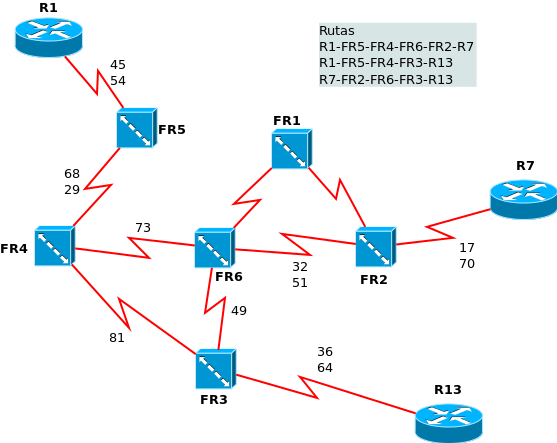
\includegraphics[scale=0.70]{diagramas/Frame_Relay.png} \\
\end{center}


\newpage
\section{Túneles GRE}
\subsection{Configuracion de los Routers}
\subsubsection{R6}
{\small
\begin{verbatim}
!
interface Ethernet0/1
 description Link to Internet
 ip address 137.43.1.2 255.255.255.252
 half-duplex
!
interface Tunnel10
 description Link to Embraer subnet (through R11)
 ip address 10.134.13.37 255.255.255.252
 tunnel source 137.43.1.2
 tunnel destination 137.43.1.6
!
interface Tunnel20
 description Link to Lockheed subnet (through R12)
 ip address 10.134.13.33 255.255.255.252
 tunnel source 137.43.1.2
 tunnel destination 137.43.1.10
!
\end{verbatim}
}

\subsubsection{R11}
{\small
\begin{verbatim}
!
interface Ethernet0/1
 description Link to Internet
 ip address 137.43.1.6 255.255.255.252
 half-duplex
!
interface Tunnel10
 description Link to Airbus subnet (through R6)
 ip address 10.134.13.38 255.255.255.252
 tunnel source 137.43.1.6
 tunnel destination 137.43.1.2
!
interface Tunnel20
 description Link to Lockheed subnet (through R12)
 ip address 10.134.13.29 255.255.255.252
 tunnel source 137.43.1.6
 tunnel destination 137.43.1.10
!
\end{verbatim}
}

\subsubsection{R12}
{\small
\begin{verbatim}
!
interface Ethernet0/1
 description Link to Internet
 ip address 137.43.1.10 255.255.255.252
 half-duplex
!
interface Tunnel10
 description Link to Airbus subnet (through R6)
 ip address 10.134.13.34 255.255.255.252
 tunnel source 137.43.1.10
 tunnel destination 137.43.1.2
!
interface Tunnel20
 description Link to Embraer subnet (through R11)
 ip address 10.134.13.30 255.255.255.252
 tunnel source 137.43.1.10
 tunnel destination 137.43.1.6
!
\end{verbatim}
}

\subsubsection{Internet}

Dentro de la topología se simuló el servicio de Internet mediante un 
router C3600.
El objetivo de la utlización del túnel GRE fue permitir el enrutamiento de 
direcciones privadas entre el par de routers que se comunican a través de 
Internet.
La configuración de los túneles GRE se basó en el apunte brindado por la 
cátedra. 

Se utilizaron tres direcciones públicas /30 para cada enlace ( R6-Internet, 
R11-Internet y R12-Internet) a partir de la dirección IP dedicada a Internet.
Luego se le asignó una direccion privada /30 para cada túnel que simula 
conectar directamente los routers R6 con R11, R6 con R12 y R11 con R12. 

Lo que finalmente se obtiene, es un encapsulamiento de un paquete IP que 
tiene como destino una dirección privada dentro de otro paquete IP con 
direccionamiento público, más la existencia de un encabezado GRE.
Los routers donde se configuran los túneles son los encargados de manipular 
estos paquetes, armándolos y desarmándolos según corresponda.

Dentro del trabajo práctico, esto se traslada a la posibilidad de que tanto 
los dispositivos y las redes existenes del lado de R6 como las de R11 puedan 
comunicarse entre sí, a pesar de que sean redes privadas con un servicio de 
Internet en el medio.
Para esto se encapsula el destino (10.134.13.xxx) con el encabezado GRE más 
otro encabezado IP con direccion pública (137.43.1.xxx).
Este paquete atraviesa internet, y al llegar al otro lado del túnel, 
el router descarta el encabezado GRE y el paquete IP con direccion pública, 
para posteriormente entregarlo a quien corresponda.

{\small
\begin{verbatim}
!
interface Ethernet0/0
 description Link to R11
 ip address 137.43.1.5 255.255.255.252
 half-duplex
!
interface Ethernet0/1
 description Link to R12
 ip address 137.43.1.9 255.255.255.252
 half-duplex
!
interface Ethernet0/2
 description Link to R6
 ip address 137.43.1.1 255.255.255.252
 half-duplex
!
\end{verbatim}
}

\subsection{Esquema del túnel GRE}
\begin{center}
	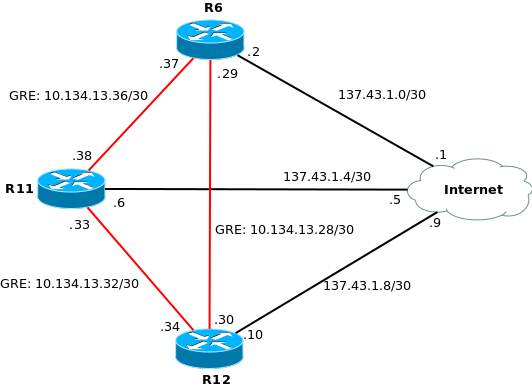
\includegraphics[scale=0.70]{diagramas/Tunel_GRE.png} \\
\end{center}

\newpage
\section{VRRP}
\subsection{Configuración de los Routers}

\subsubsection{Sede Chos Malal}
\paragraph{R4}
{\small
\begin{verbatim}

\end{verbatim}

\paragraph{R5}
{\small
\begin{verbatim}

\end{verbatim}
}

\subsubsection{Sede Junín de los Andes}
\paragraph{R8}
{\small
\begin{verbatim}

\end{verbatim}
}

\paragraph{R9}
{\small
\begin{verbatim}

\end{verbatim}
}

\section{OSPF}
Se implementó OSPF para ruteo dinámico en la sede Junín de los Andes.

Los routers distribuyen sus rutas estáticas en las actualizaciones LS Update 
que envían.
Para evitar que envíen dicha información más allá de los límites de la sede, 
se pasivaron las interfaces correspondientes de aquellos routers en los bordes.

\subsection{Configuración de los Routers}
\subsubsection{R7}
{\small
\begin{verbatim}
!
router ospf 100
 log-adjacency-changes
 redistribute static subnets
 passive-interface Ethernet0/0
 passive-interface Ethernet0/1
 network 10.134.1.0 0.0.0.255 area 0
 network 172.13.1.192  0.0.0.3 area 0
 network 172.13.1.200  0.0.0.3 area 0
 network 10.134.13.44  0.0.0.3 area 0
!
\end{verbatim}
}

\subsubsection{R8}
{\small
\begin{verbatim}
!
router ospf 100
 log-adjacency-changes
 redistribute static
 network 10.134.1.0 0.0.0.255 area 0
 network 10.134.13.128  0.0.0.31 area 0
!
\end{verbatim}
}

\subsubsection{R9}
{\small
\begin{verbatim}
!
router ospf 100
 log-adjacency-changes
 redistribute static subnets
 passive-interface Ethernet0/2
 network 10.134.1.0 0.0.0.255 area 0
 network 10.134.13.40  0.0.0.3 area 0
 network 10.134.13.128  0.0.0.31 area 0
 network 10.134.5.128 0.0.0.127 area 0
!
\end{verbatim}
}

\subsubsection{R10}
{\small
\begin{verbatim}
!
router ospf 100
 log-adjacency-changes
 redistribute static
 network 10.134.5.128 0.0.0.127 area 0
 network 10.134.13.96  0.0.0.31 area 0
!
\end{verbatim}
}

\subsubsection{R11}
{\small
\begin{verbatim}
!
router ospf 100
 log-adjacency-changes
 redistribute static subnets
 passive-interface Tunnel10
 passive-interface Tunnel20
 passive-interface Ethernet0/1
 network 10.134.5.128 0.0.0.127 area 0
 network 10.134.13.36  0.0.0.3 area 0
 network 10.134.13.28  0.0.0.3 area 0
!
\end{verbatim}
}

\newpage
\section{DNS}
Para obtener la ip asociado a un nombre(o viceversa), cada host realiza 
la solicitud a su servidor DNS local, que corresponde a la zona en la que 
se encuentre.
En la sede Chos Malal se corresponde el DNS 1 y para Junín de los Andes y 
Alumine corresponde el DNS 2.
Cuando un servidor DNS no conoce un nombre de dominio y posee el mismo 
dominio de la empresa, este realiza una solicitud al DNS root que le responde 
con la dirección del otro servidor DNS para así consultar por la respuesta de 
la solicitud inicial, y esta manera se resolvería la solicitud de forma 
iterativa.

Para la resolución de nombres de dominio y distinguir los diferentes hosts 
pertenecientes a cada sede, se agregaron dominios con el nombre de la sede 
al dominio que ya posee la empresa (neuquen.dc.fi.uba.ar).
Un ejemplo sería, para el host A que se encuentra en al Red C (denominada 
como Concorde) perteneciente a la sede Chos Malal, su dominio asociado sería 
a.chosmalal.neuquen.dc.fi.uba.ar.
Otro ejemplo podría ser del servidor FTP, que se encuentra en la red B 
(denominada como Boeing) en la sede Alumine con el nombre asociado de 
ftp.alumine.neuquen.dc.fi.uba.ar.

\section{OPEN VPN}
Se crearon 7 VPNs, una para cada red conectada a dispositivos físicos.

\subsection{Servers}
Los 7 VPN servers corren en paralelo en 7 puertos diferentes, en la misma PC 
que tiene la topología.
Para cada uno, está configurada una interfaz tap en modo promiscuo, la cual 
escucha todos los paquetes que llegan.
A través de NIO ethernet, se encuentran conectadas dichas interfaces a la LAN 
de la topología correspondiente.

\subsection{Clientes}
Para cada cliente, existe un script que configura la conexión y 
las rutas del dispositivo (i.e. su default gateway) para crear el VPN.

\newpage
\section{Anexo}
\subsection{Topología}
\begin{figure}[h!]
	\centering
	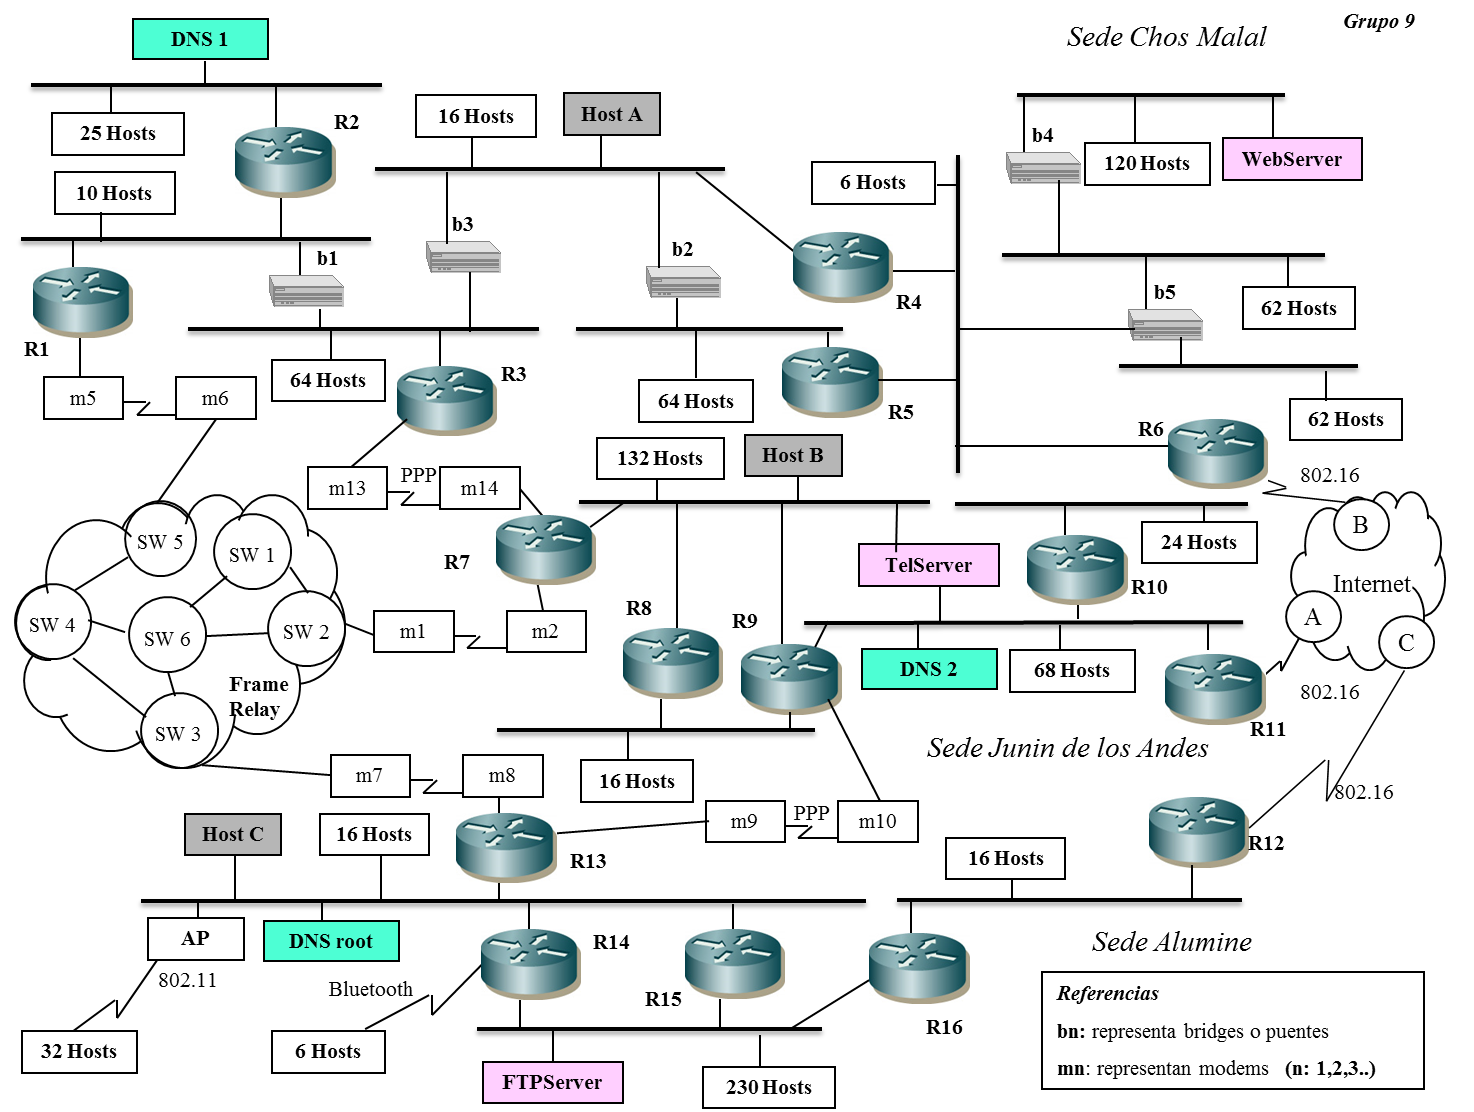
\includegraphics[scale=0.45,angle=90]{diagramas/topologia.png} \\
\end{figure}

\subsection{Topología con redes marcadas}
\begin{figure}[h!]
	\centering
	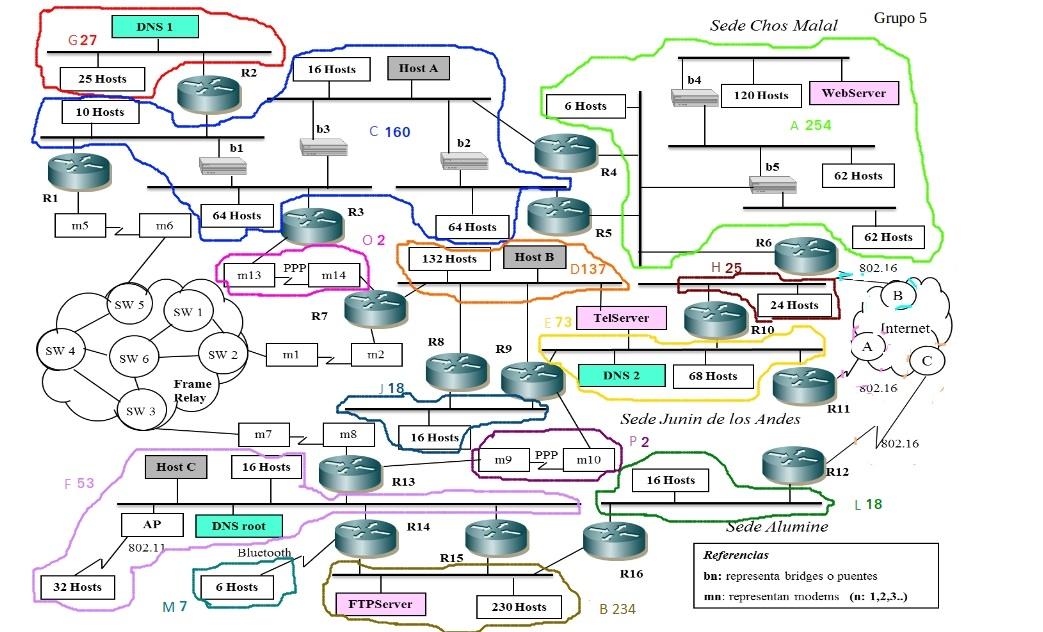
\includegraphics[scale=0.85,angle=90]{diagramas/topologia_marcada.jpg} \\
\end{figure}

%\subsection{Esquema de la topología}
%	\includegraphics[scale=0.35,angle=90]{./TopologiaEsquema.png}~\\
%\end{figure}

\end{document}